
%% bare_conf.tex
%% V1.3
%% 2007/01/11
%% by Michael Shell
%% See:
%% http://www.michaelshell.org/
%% for current contact information.
%%
%% This is a skeleton file demonstrating the use of IEEEtran.cls
%% (requires IEEEtran.cls version 1.7 or later) with an IEEE conference paper.
%%
%% Support sites:
%% http://www.michaelshell.org/tex/ieeetran/
%% http://www.ctan.org/tex-archive/macros/latex/contrib/IEEEtran/
%% and
%% http://www.ieee.org/

%%*************************************************************************
%% Legal Notice:
%% This code is offered as-is without any warranty either expressed or
%% implied; without even the implied warranty of MERCHANTABILITY or
%% FITNESS FOR A PARTICULAR PURPOSE! 
%% User assumes all risk.
%% In no event shall IEEE or any contributor to this code be liable for
%% any damages or losses, including, but not limited to, incidental,
%% consequential, or any other damages, resulting from the use or misuse
%% of any information contained here.
%%
%% All comments are the opinions of their respective authors and are not
%% necessarily endorsed by the IEEE.
%%
%% This work is distributed under the LaTeX Project Public License (LPPL)
%% ( http://www.latex-project.org/ ) version 1.3, and may be freely used,
%% distributed and modified. A copy of the LPPL, version 1.3, is included
%% in the base LaTeX documentation of all distributions of LaTeX released
%% 2003/12/01 or later.
%% Retain all contribution notices and credits.
%% ** Modified files should be clearly indicated as such, including  **
%% ** renaming them and changing author support contact information. **
%%
%% File list of work: IEEEtran.cls, IEEEtran_HOWTO.pdf, bare_adv.tex,
%%                    bare_conf.tex, bare_jrnl.tex, bare_jrnl_compsoc.tex
%%*************************************************************************

% *** Authors should verify (and, if needed, correct) their LaTeX system  ***
% *** with the testflow diagnostic prior to trusting their LaTeX platform ***
% *** with production work. IEEE's font choices can trigger bugs that do  ***
% *** not appear when using other class files.                            ***
% The testflow support page is at:
% http://www.michaelshell.org/tex/testflow/



% Note that the a4paper option is mainly intended so that authors in
% countries using A4 can easily print to A4 and see how their papers will
% look in print - the typesetting of the document will not typically be
% affected with changes in paper size (but the bottom and side margins will).
% Use the testflow package mentioned above to verify correct handling of
% both paper sizes by the user's LaTeX system.
%
% Also note that the "draftcls" or "draftclsnofoot", not "draft", option
% should be used if it is desired that the figures are to be displayed in
% draft mode.
%
\documentclass[conference]{IEEEtran}
% Add the compsoc option for Computer Society conferences.
%
% If IEEEtran.cls has not been installed into the LaTeX system files,
% manually specify the path to it like:
% \documentclass[conference]{../sty/IEEEtran}





% Some very useful LaTeX packages include:
% (uncomment the ones you want to load)


% *** MISC UTILITY PACKAGES ***
%
%\usepackage{ifpdf}
% Heiko Oberdiek's ifpdf.sty is very useful if you need conditional
% compilation based on whether the output is pdf or dvi.
% usage:
% \ifpdf
%   % pdf code
% \else
%   % dvi code
% \fi
% The latest version of ifpdf.sty can be obtained from:
% http://www.ctan.org/tex-archive/macros/latex/contrib/oberdiek/
% Also, note that IEEEtran.cls V1.7 and later provides a builtin
% \ifCLASSINFOpdf conditional that works the same way.
% When switching from latex to pdflatex and vice-versa, the compiler may
% have to be run twice to clear warning/error messages.






% *** CITATION PACKAGES ***
%
%\usepackage{cite}
% cite.sty was written by Donald Arseneau
% V1.6 and later of IEEEtran pre-defines the format of the cite.sty package
% \cite{} output to follow that of IEEE. Loading the cite package will
% result in citation numbers being automatically sorted and properly
% "compressed/ranged". e.g., [1], [9], [2], [7], [5], [6] without using
% cite.sty will become [1], [2], [5]--[7], [9] using cite.sty. cite.sty's
% \cite will automatically add leading space, if needed. Use cite.sty's
% noadjust option (cite.sty V3.8 and later) if you want to turn this off.
% cite.sty is already installed on most LaTeX systems. Be sure and use
% version 4.0 (2003-05-27) and later if using hyperref.sty. cite.sty does
% not currently provide for hyperlinked citations.
% The latest version can be obtained at:
% http://www.ctan.org/tex-archive/macros/latex/contrib/cite/
% The documentation is contained in the cite.sty file itself.


\usepackage{enumerate}
\usepackage{rotating}


% *** GRAPHICS RELATED PACKAGES ***
%
\ifCLASSINFOpdf
  % \usepackage[pdftex]{graphicx}
  % declare the path(s) where your graphic files are
  % \graphicspath{{../pdf/}{../jpeg/}}
  % and their extensions so you won't have to specify these with
  % every instance of \includegraphics
  % \DeclareGraphicsExtensions{.pdf,.jpeg,.png}
\else
  % or other class option (dvipsone, dvipdf, if not using dvips). graphicx
  % will default to the driver specified in the system graphics.cfg if no
  % driver is specified.
  % \usepackage[dvips]{graphicx}
  % declare the path(s) where your graphic files are
  % \graphicspath{{../eps/}}
  % and their extensions so you won't have to specify these with
  % every instance of \includegraphics
  % \DeclareGraphicsExtensions{.eps}
\fi
% graphicx was written by David Carlisle and Sebastian Rahtz. It is
% required if you want graphics, photos, etc. graphicx.sty is already
% installed on most LaTeX systems. The latest version and documentation can
% be obtained at: 
% http://www.ctan.org/tex-archive/macros/latex/required/graphics/
% Another good source of documentation is "Using Imported Graphics in
% LaTeX2e" by Keith Reckdahl which can be found as epslatex.ps or
% epslatex.pdf at: http://www.ctan.org/tex-archive/info/
%
% latex, and pdflatex in dvi mode, support graphics in encapsulated
% postscript (.eps) format. pdflatex in pdf mode supports graphics
% in .pdf, .jpeg, .png and .mps (metapost) formats. Users should ensure
% that all non-photo figures use a vector format (.eps, .pdf, .mps) and
% not a bitmapped formats (.jpeg, .png). IEEE frowns on bitmapped formats
% which can result in "jaggedy"/blurry rendering of lines and letters as
% well as large increases in file sizes.
%
% You can find documentation about the pdfTeX application at:
% http://www.tug.org/applications/pdftex





% *** MATH PACKAGES ***
%
%\usepackage[cmex10]{amsmath}
% A popular package from the American Mathematical Society that provides
% many useful and powerful commands for dealing with mathematics. If using
% it, be sure to load this package with the cmex10 option to ensure that
% only type 1 fonts will utilized at all point sizes. Without this option,
% it is possible that some math symbols, particularly those within
% footnotes, will be rendered in bitmap form which will result in a
% document that can not be IEEE Xplore compliant!
%
% Also, note that the amsmath package sets \interdisplaylinepenalty to 10000
% thus preventing page breaks from occurring within multiline equations. Use:
%\interdisplaylinepenalty=2500
% after loading amsmath to restore such page breaks as IEEEtran.cls normally
% does. amsmath.sty is already installed on most LaTeX systems. The latest
% version and documentation can be obtained at:
% http://www.ctan.org/tex-archive/macros/latex/required/amslatex/math/





% *** SPECIALIZED LIST PACKAGES ***
%
%\usepackage{algorithmic}
% algorithmic.sty was written by Peter Williams and Rogerio Brito.
% This package provides an algorithmic environment fo describing algorithms.
% You can use the algorithmic environment in-text or within a figure
% environment to provide for a floating algorithm. Do NOT use the algorithm
% floating environment provided by algorithm.sty (by the same authors) or
% algorithm2e.sty (by Christophe Fiorio) as IEEE does not use dedicated
% algorithm float types and packages that provide these will not provide
% correct IEEE style captions. The latest version and documentation of
% algorithmic.sty can be obtained at:
% http://www.ctan.org/tex-archive/macros/latex/contrib/algorithms/
% There is also a support site at:
% http://algorithms.berlios.de/index.html
% Also of interest may be the (relatively newer and more customizable)
% algorithmicx.sty package by Szasz Janos:
% http://www.ctan.org/tex-archive/macros/latex/contrib/algorithmicx/




% *** ALIGNMENT PACKAGES ***
%
%\usepackage{array}
% Frank Mittelbach's and David Carlisle's array.sty patches and improves
% the standard LaTeX2e array and tabular environments to provide better
% appearance and additional user controls. As the default LaTeX2e table
% generation code is lacking to the point of almost being broken with
% respect to the quality of the end results, all users are strongly
% advised to use an enhanced (at the very least that provided by array.sty)
% set of table tools. array.sty is already installed on most systems. The
% latest version and documentation can be obtained at:
% http://www.ctan.org/tex-archive/macros/latex/required/tools/


%\usepackage{mdwmath}
%\usepackage{mdwtab}
% Also highly recommended is Mark Wooding's extremely powerful MDW tools,
% especially mdwmath.sty and mdwtab.sty which are used to format equations
% and tables, respectively. The MDWtools set is already installed on most
% LaTeX systems. The lastest version and documentation is available at:
% http://www.ctan.org/tex-archive/macros/latex/contrib/mdwtools/


% IEEEtran contains the IEEEeqnarray family of commands that can be used to
% generate multiline equations as well as matrices, tables, etc., of high
% quality.


%\usepackage{eqparbox}
% Also of notable interest is Scott Pakin's eqparbox package for creating
% (automatically sized) equal width boxes - aka "natural width parboxes".
% Available at:
% http://www.ctan.org/tex-archive/macros/latex/contrib/eqparbox/





% *** SUBFIGURE PACKAGES ***
%\usepackage[tight,footnotesize]{subfigure}
% subfigure.sty was written by Steven Douglas Cochran. This package makes it
% easy to put subfigures in your figures. e.g., "Figure 1a and 1b". For IEEE
% work, it is a good idea to load it with the tight package option to reduce
% the amount of white space around the subfigures. subfigure.sty is already
% installed on most LaTeX systems. The latest version and documentation can
% be obtained at:
% http://www.ctan.org/tex-archive/obsolete/macros/latex/contrib/subfigure/
% subfigure.sty has been superceeded by subfig.sty.



%\usepackage[caption=false]{caption}
%\usepackage[font=footnotesize]{subfig}
% subfig.sty, also written by Steven Douglas Cochran, is the modern
% replacement for subfigure.sty. However, subfig.sty requires and
% automatically loads Axel Sommerfeldt's caption.sty which will override
% IEEEtran.cls handling of captions and this will result in nonIEEE style
% figure/table captions. To prevent this problem, be sure and preload
% caption.sty with its "caption=false" package option. This is will preserve
% IEEEtran.cls handing of captions. Version 1.3 (2005/06/28) and later 
% (recommended due to many improvements over 1.2) of subfig.sty supports
% the caption=false option directly:
%\usepackage[caption=false,font=footnotesize]{subfig}
%
% The latest version and documentation can be obtained at:
% http://www.ctan.org/tex-archive/macros/latex/contrib/subfig/
% The latest version and documentation of caption.sty can be obtained at:
% http://www.ctan.org/tex-archive/macros/latex/contrib/caption/




% *** FLOAT PACKAGES ***
%
%\usepackage{fixltx2e}
% fixltx2e, the successor to the earlier fix2col.sty, was written by
% Frank Mittelbach and David Carlisle. This package corrects a few problems
% in the LaTeX2e kernel, the most notable of which is that in current
% LaTeX2e releases, the ordering of single and double column floats is not
% guaranteed to be preserved. Thus, an unpatched LaTeX2e can allow a
% single column figure to be placed prior to an earlier double column
% figure. The latest version and documentation can be found at:
% http://www.ctan.org/tex-archive/macros/latex/base/



%\usepackage{stfloats}
% stfloats.sty was written by Sigitas Tolusis. This package gives LaTeX2e
% the ability to do double column floats at the bottom of the page as well
% as the top. (e.g., "\begin{figure*}[!b]" is not normally possible in
% LaTeX2e). It also provides a command:
%\fnbelowfloat
% to enable the placement of footnotes below bottom floats (the standard
% LaTeX2e kernel puts them above bottom floats). This is an invasive package
% which rewrites many portions of the LaTeX2e float routines. It may not work
% with other packages that modify the LaTeX2e float routines. The latest
% version and documentation can be obtained at:
% http://www.ctan.org/tex-archive/macros/latex/contrib/sttools/
% Documentation is contained in the stfloats.sty comments as well as in the
% presfull.pdf file. Do not use the stfloats baselinefloat ability as IEEE
% does not allow \baselineskip to stretch. Authors submitting work to the
% IEEE should note that IEEE rarely uses double column equations and
% that authors should try to avoid such use. Do not be tempted to use the
% cuted.sty or midfloat.sty packages (also by Sigitas Tolusis) as IEEE does
% not format its papers in such ways.





% *** PDF, URL AND HYPERLINK PACKAGES ***
%
%\usepackage{url}
% url.sty was written by Donald Arseneau. It provides better support for
% handling and breaking URLs. url.sty is already installed on most LaTeX
% systems. The latest version can be obtained at:
% http://www.ctan.org/tex-archive/macros/latex/contrib/misc/
% Read the url.sty source comments for usage information. Basically,
% \url{my_url_here}.





% *** Do not adjust lengths that control margins, column widths, etc. ***
% *** Do not use packages that alter fonts (such as pslatex).         ***
% There should be no need to do such things with IEEEtran.cls V1.6 and later.
% (Unless specifically asked to do so by the journal or conference you plan
% to submit to, of course. )


% correct bad hyphenation here
\hyphenation{op-tical net-works semi-conduc-tor}


\begin{document}
%
% paper title
% can use linebreaks \\ within to get better formatting as desired
\title{Usability Criteria for Graphical Code Completion}


% author names and affiliations
% use a multiple column layout for up to three different
% affiliations
\author{\IEEEauthorblockN{Cyrus Omar}
\IEEEauthorblockA{Computer Science Department\\
Carnegie Mellon University\\
Pittsburgh, PA 15213\\
cyrus@cmu.edu}
\and
\IEEEauthorblockN{YoungSeok Yoon}
\IEEEauthorblockA{Institute for Software Research\\
Carnegie Mellon University\\
Pittsburgh, PA 15213\\
youngseok@cs.cmu.edu}
}

% conference papers do not typically use \thanks and this command
% is locked out in conference mode. If really needed, such as for
% the acknowledgment of grants, issue a \IEEEoverridecommandlockouts
% after \documentclass

% for over three affiliations, or if they all won't fit within the width
% of the page, use this alternative format:
% 
%\author{\IEEEauthorblockN{Michael Shell\IEEEauthorrefmark{1},
%Homer Simpson\IEEEauthorrefmark{2},
%James Kirk\IEEEauthorrefmark{3}, 
%Montgomery Scott\IEEEauthorrefmark{3} and
%Eldon Tyrell\IEEEauthorrefmark{4}}
%\IEEEauthorblockA{\IEEEauthorrefmark{1}School of Electrical and Computer Engineering\\
%Georgia Institute of Technology,
%Atlanta, Georgia 30332--0250\\ Email: see http://www.michaelshell.org/contact.html}
%\IEEEauthorblockA{\IEEEauthorrefmark{2}Twentieth Century Fox, Springfield, USA\\
%Email: homer@thesimpsons.com}
%\IEEEauthorblockA{\IEEEauthorrefmark{3}Starfleet Academy, San Francisco, California 96678-2391\\
%Telephone: (800) 555--1212, Fax: (888) 555--1212}
%\IEEEauthorblockA{\IEEEauthorrefmark{4}Tyrell Inc., 123 Replicant Street, Los Angeles, California 90210--4321}}




% use for special paper notices
%\IEEEspecialpapernotice{(Invited Paper)}




% make the title area
\maketitle


%\begin{abstract}
%\boldmath
%\end{abstract}
% IEEEtran.cls defaults to using nonbold math in the Abstract.
% This preserves the distinction between vectors and scalars. However,
% if the conference you are submitting to favors bold math in the abstract,
% then you can use LaTeX's standard command \boldmath at the very start
% of the abstract to achieve this. Many IEEE journals/conferences frown on
% math in the abstract anyway.

% no keywords




% For peer review papers, you can put extra information on the cover
% page as needed:
% \ifCLASSOPTIONpeerreview
% \begin{center} \bfseries EDICS Category: 3-BBND \end{center}
% \fi
%
% For peerreview papers, this IEEEtran command inserts a page break and
% creates the second title. It will be ignored for other modes.
\IEEEpeerreviewmaketitle



\section{Introduction}
Many source code editors today feature interactive code completion. By invoking a keyboard shortcut, developers can summon a floating palette containing a list of contextually relevant variables, fields, methods, classes and code snippets. An adjacent floating window displays documentation for the currently highlighted item. This interface helps developers explore APIs and avoid basic spelling and logic errors [?], and empirical data indicates that professional developers invoke interactive code completion frequently \cite{murphy_how_2006}. 

A number of new to the code completion list have been proposed in the literature. These methods combine information about the program context with make use of usage history [?], examples extracted from code repositories [?, ?] and crowdsourced information [?] 

Calcite, reordering, crowdsourced code completion papers.

Our proposal: graphical code completion. Inversion of control: look at class. Also possible to look at external database. Visual languages have shown this might be useful in certain circumstances (?).

Consistent with best practices, we begin by seeking the usability criteria that govern whether such a system would be useful to professional developers. We conducted a large survey of these developers and extracted several criteria that both constrain the overall system architecture and inform the design (or caution against designing) palettes for different kinds of classes.

%\section{Tool}
%Described earlier.

\section{Methods}
Our subject pool consisted primarily of visitors to a large collaborative filtering website dedicated to programming called {\tt /r/programming} on reddit.com\footnote{http://www.reddit.com/r/programming}. At the time of our study, there were approximately 340,000 registered members. A small number of participants were also recruited using a mass email to local computer science graduate students. The recruitment materials in both cases stated that we were seeking developers ''familiar with an object-oriented programming language like Java, C\# or Visual Basic and an integrated development environment like Eclipse or Visual Studio''.

Participants were asked to take an online survey that would take approximately 20 minutes to complete. Of the 696 participants who started the survey, 475 participants finished it. Of these, 457 participants came from /r/programming and 18 from the graduate student mailing list. All quantitative metrics used in this study are based only on these participants.

\subsection{Familiarity with Languages and Editors}

We began by asking participants to rate their level of familiarity with several programming languages. Figure 1 summarizes these ratings. On average, participants rated themselves as very familiar with Java, C, C++ and JavaScript, familiar with C\#, Python and PHP and somewhat familiar with Visual Basic and Perl.

We also asked participants to select the integrated development environments and code editors that they were familiar with. The Eclipse IDE was familiar to 87.1\% of participants. This was followed by Visual Studio with 66.0\% of participants, Vi/Vim with 53.7\%, Netbeans with 37.7\%, Emacs with 24.8\% and IntelliJ IDEA with 16.4\%. Participants could also enter ``other'' choices. A number of editors and IDEs were entered, including Xcode, Textmate, Notepad++ and others.
%\begin{figure}
%  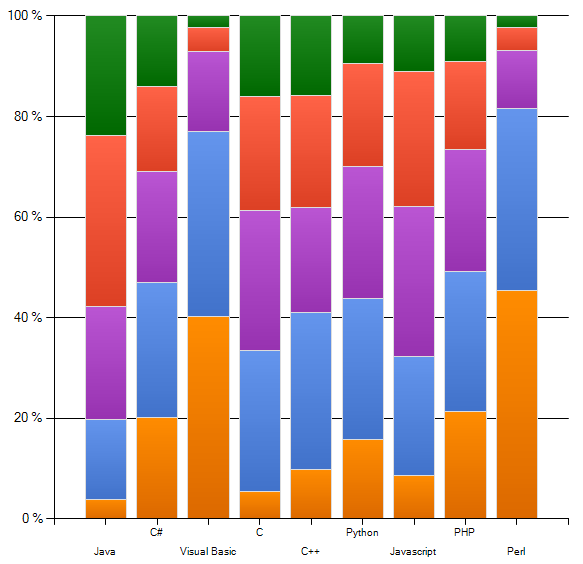
\includegraphics[width=3.5in,height=2in]{experience.png}
%  \caption{Participant familiarity with various programming languages. Starting at bottom: None, Somewhat familiar, Familiar, Very Familiar, Expert.}
%\end{figure}

\subsection{Mockups}
\begin{figure*}
  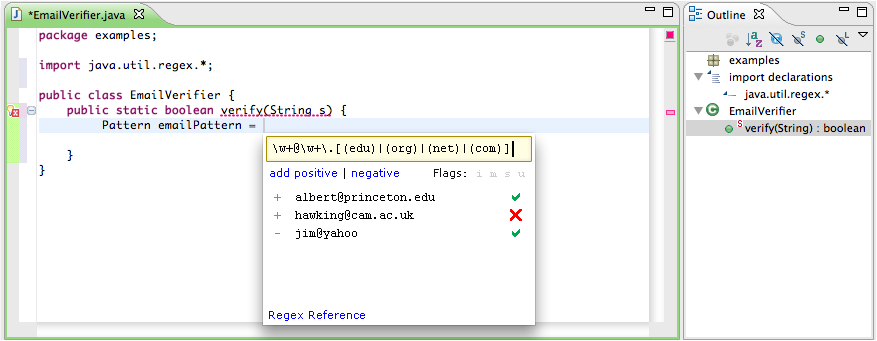
\includegraphics[scale=.6]{mockup-palette.png}
  \caption{The regular expression palette, shown in Eclipse.}
\end{figure*}
Next, we presented participants with a series of mockup palettes corresponding to a Color class, a regular expression Pattern class (Figure 2) and a SQL query ResultSet class. In addition to a screenshot of the palette itself, participants were shown mockups demonstrating how a user would invoke the palette, and a mockup showing the code that would be inserted once a selection had been made. 

Before presenting each palette mockup we gathered information about the user's familiarity with that topic and the strategies that they would likely use to instantiate that class. The Color class was presumed familiar to all participants. Figure 3 summarizes responses for the regular expression and SQL classes. The low number of participants unfamiliar with these topics again provides evidence that our participants were not generally novice developers.

To determine the strategy typically used for instantiating the Color class, we asked the following question. The values in bold show the frequency of each response.

\begin{quote}
A user interface designer asks you to change the background color of a window to ``navy blue'' when the user presses a button. You have determined that you need to instantiate the 'Color' class to do so.
\\\\
Which of the following strategies would you use first to create an instance of the 'Color' class representing navy blue?\\

\begin{enumerate}[(a)]
\item I would use the IDE's content assist menu (see note below) to look for a predefined constant representing navy blue. (\textbf{58.4\%})
\item I would look up the documentation of the Color class to see if there is a predefined constant representing navy blue. (\textbf{19.0\%})
\item I would use an external tool (e.g. Photoshop or some other image editor) to determine the RGB values for navy blue. (\textbf{14.0\%})
\item I would guess at the RGB values for navy blue, then check whether my guess was correct by executing the application. (\textbf{5.3\%})
\item Other (please specify) (\textbf{3.3\%})\\
\end{enumerate}
\end{quote}

Figure 4 summarizes the responses to a more general question asked about regular expressions and SQL queries.

\begin{figure}
\begin{tabular}{lccc}
 & \textbf{Regular Expressions} &  & \textbf{SQL}\\
 \hline
Never used & 4.8\% &  & 0.0\%\\
Use infrequently & 46.7\% &  & 37.4\%\\
Use frequently & \textbf{48.4\%} &  & \textbf{62.6\%}\\
\hline
\end{tabular}
\caption{Participant's experience with regular expressions and SQL.}
\end{figure}

\begin{figure}
\begin{tabular}{lccc}
 & \textbf{Regular Expressions} &  & \textbf{SQL}\\
 \hline
Separate test script & 29.7\% &  & 15.5\%\\
Guess and check & 13.4\% &  & 16.0\%\\
External tool & \textbf{38.5\%} &  & \textbf{58.9\%}\\
Search for examples & 12.1\% & & 4.8\% \\
Other & 6.2\% & & 4.8\% \\
\hline
\end{tabular}
\caption{Typical strategies for regular expressions and SQL queries.}
\end{figure}


%For each of these classes,


%\subsubsection{Color}
%We began with a class representing colors. We asked participants to consider the following scenario:

\begin{figure}
\begin{tabular}{crccccc}\\\\
\textsc{class}
& 
& \begin{rotate}{20}Nearly every time\end{rotate}
& \begin{rotate}{20}Most of the time\end{rotate}
& \begin{rotate}{20}Some of the time\end{rotate}
& \begin{rotate}{20}Rarely\end{rotate}
& \begin{turn}{20}Never\end{turn}\\
\hline
Color &\vline& 9.6\% & 22.1\% & \textbf{32.4\%} & 28.2\% & 7.7\%\\
RegExp &\vline& \textbf{36.6\%} & 29.5\% & 21.8\% & 7.3\% & 4.8\%\\
SQL & \vline &18.2\% & 19.3\% & \textbf{30.9\%} & 20.4\% & 11.4\%\\
\hline
\end{tabular}
\caption{For each of the classes considered, participants were shown mockups of a code completion palette designed for instantiating that class, as well as the source code generated after parameters were entered. This table shows the distribution of responses to the question: ``Consider situations where you need to instantiate the [specified] class. What portion of the time, in these situations, do you think you would use this feature?''}
\end{figure}
%
%\begin{figure}
%  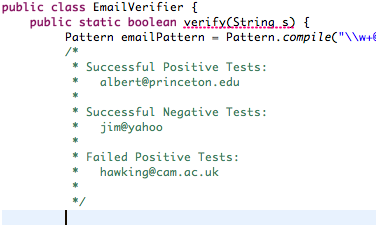
\includegraphics[scale=.6]{regex-insert.png}
%  \caption{Test}
%\end{figure}
%
%

%Then we asked:
%\begin{quote}
%\textbf{Q2} Consider situations where you need to instantiate the 'Color' class. What portion of the time, in these situations, do you think you would use this feature?
%\begin{enumerate}[(a)]
%\item Nearly every time (\textbf{9.6\%})
%\item Most of the time (\textbf{22.1\%})
%\item Some of the time (\textbf{32.4\%})
%\item Rarely (\textbf{28.2\%})
%\item Never (\textbf{7.7\%})\\
%\end{enumerate}
%\end{quote}
%

After presenting each palette, we asked users to rate the usefulness of each palette. Responses are summarized in Figure 5. We then allowed participants to provide qualifications and open-ended feedback by asking the following question: ``If you would like to qualify or elaborate on your answer to the previous question you may do so below. You may also suggest improvements for this palette.'' This information is analyzed in the remainder of the paper.

%\begin{quote}
%\textbf{Q4} How would you describe your level of familiarity with (regular expressions, SQL)?\\
%\\
%\begin{enumerate}[(a)]
%\item I do not know what [it is].	 (\textbf{0.7\%}, \textbf{0.0\%})
%\item I know what regular expressions are but I have not used them in practice. (\textbf{4.4\%, 0.0\%})
%\item I use regular expressions infrequently.	 (\textbf{46.0\%, 35.9\%})
%\item I use regular expressions frequently. (\textbf{49.0\%, 64.1\%})
%\end{enumerate}
%\end{quote}



%\begin{quote}
%\textbf{Q5} Consider situations where you need to write a regular expression to extract information from a string or collection of strings. What strategy would you most likely use first?

%\begin{enumerate}[(a)]
%\item I would write a separate test script to help come up with an appropriate regular expression. (\textbf{29.7\%})
%\item I would guess and check regular expressions by running my application. (\textbf{13.4\%})
%\item I would launch an external application or web tool to help me test regular expressions interactively. (\textbf{38.5\%})
%\item I would search the web for a sample regular expression suitable for my task. (\textbf{12.1\%})
%\item Other (please specify) (\textbf{6.2\%})
%\end{enumerate}
%\end{quote}


%\begin{quote}
%\textbf{Q6} Consider situations where you need to create a regular expression. What portion of the time, in these situations, do you think you would use this feature?
%\begin{enumerate}[(a)]
%\item Nearly every time (\textbf{36.6\%})
%\item Most of the time (\textbf{29.5\%})
%\item Some of the time (\textbf{21.8\%})
%\item Rarely (\textbf{7.3\%})
%\item Never (\textbf{4.8\%})\\
%\end{enumerate}
%\end{quote}

%\begin{quote}
%\textbf{Q7} How would you describe your level of familiarity with SQL?

%\begin{enumerate}[(a)]
%\item I do not know what regular expressions are.	 (\textbf{0.0\%})
%\item I know what SQL is I have not used it in practice. (\textbf{0.0\%})
%\item I use SQL infrequently.	 (\textbf{35.9\%})
%\item I use SQL frequently. (\textbf{64.1\%})\\
%\end{enumerate}
%\end{quote}

%\begin{quote}
%\textbf{Q8} Consider situations where you need to write a regular expression to extract information from a string or collection of strings. What strategy would you most likely use first?

%\begin{enumerate}[(a)]
%\item I would write a separate test script to help come up with an appropriate SQL query.	
 %(\textbf{15.5\%})
%\item I would guess and check by running my application. (\textbf{16.0\%})
%\item I would launch an external application or web tool to test my query against my database interactively.	(\textbf{58.9\%})
%\item I would search the web for an example SQL query suitable for my task.	
 %(\textbf{4.8\%})
%\item Other (please specify) (\textbf{4.8\%})
%\end{enumerate}
%\end{quote}

%Showed the SQL palette and asked:

%\begin{quote}
%\textbf{Q9} Consider situations where you need to create a SQL query. How often, in these situations, do you think you would use this feature?
%\end{quote}

\section{Design Implications}
\begin{figure}[b]
  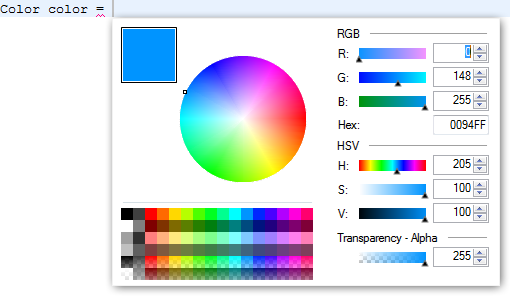
\includegraphics[scale=.5]{color-palette.png}
  \caption{test}
\end{figure}

We next analyzed the open-ended responses to extract some design principles and constraints. We got 193 responses for the color palette, 129 for the regular expression palette, and 142 for the SQL palette. Also, we got total 119 suggestions about what other types of classes could benefit from similar types of palettes. The design can be divided into two main categories: system design constraints, and general palette design considerations. System design constraints are the criteria that should be taken into account in the design of the overall system architecture, and the general palette design considerations are about how to make more usable palettes.

\subsection{System Design Constraints}

\subsubsection{Handling Separation of Concerns}

Professional developers were very wary of including constant data into the source code directly. Many responses expressed general sentiment or specific preference for project-wide color theme or external resource file. Also, many people stated that these tools might not be useful since they usually read an external resource file, or sometimes they explicitly suggested to add capability to handle the external resource files directly from the palette.

Examples of feedbacks in this category include:

\begin{itemize}
	\item The use of magic numbers in the source code is a bad design (54)
	\item Color picking is the `designer's job' (33)
	\item Would only use to define named constants (17)
	\item Would rather use color scheme / theme (3)
	\item Would use Object-Relational Mapping (ORM) / Language INtegrated Query (LINQ) instead of raw SQL query string (27 of 142)
	\item These palettes might be useful for prototyping, but not for real production (14)
	\item Instead of including the test cases into comments, they should be stored as unit tests (35 of 143)
\end{itemize}

Interestingly, most people seemed to consider regular expressions as part of the program logic. There were few people who complained about including the regular expression pattern string in the source code.
 
\subsubsection{Reversibility}

19 participants expressed that it should be able to bring the palettes back when they want to modify the parameters after they used the palettes.
 
\subsubsection{Palette Settings and State}

Many participants wanted to be able to configure the palettes or have the palettes maintain state even after the palettes are hidden. The followings are the comments that are related to this category.

\begin{itemize}
	\item Want recently used regular expressions, and control over the comments (12)
	\item Persistent database connection information is needed / want to manage connection pools (9)
	\item Want recent colors, capability of setting favorite colors (20)
\end{itemize}

\subsubsection{Interaction with Code Context}

Some people wanted to interact with the code context. For example, 13 people expressed that it would be great if the SQL query palette was capable of dynamically creating SQL query string by combining multiple string variables, or by assigning variables for the parameters.

\subsubsection{Performance}

Developers were concerned about the performance of these palettes. Some of the participants said that they would use these palettes only if it does not slow down the IDE. Also, this was the most popular comment on the reddit thread.

\subsubsection{IDE Independence}

Several participants expressed a desire for IDE or even language independence for these palettes.

%\subsubsection{Composing palette logic}

\subsection{General Palette Design Considerations}
\subsubsection{Simplicity vs. Capability}

Even though the participants were shown the same mockup screenshots, their reactions were split. Our color palette was considered too complex by many participants (26), and many others (26) would be satisfied with seeing colors next to a list of color names. The regular expressoin palette and SQL palette were considered too simple (12, and 15 participants respectively). They wanted syntax highlighting, match highlighting, and browsing capability of SQL databases.

\subsubsection{Keyboard Navigability}

12 of the participants expressed strong antipathy toward the mouse. This was mostly directed at the color palette.

\subsubsection{Complexity}

%\subsubsection{Side Effects}

\section{Suggestions from the Participants}
We classified the suggestions into several categories. The number in the parentheses indicate the number of participants who suggested the classes which fall into the category.

\subsection{Alternative/Tricky/Literal Syntax (16)}
These are the classes of which syntax is tricky, or complex. Even for a basic string class, people wanted to input multiline string or unicode string in more convenient way with automatic escaping.

\begin{itemize}
	\item Example classes
	
	\begin{itemize}
		\item String
		\item Collections (e.g., dictionary)
		\item Vector, Matrix
		\item Embedded languages
		\item URLs, Paths
	\end{itemize}
	
	\item Expected features
	
	\begin{itemize}
		\item Proper escaping
		\item Syntax highlighting
		\item Auto-completion
	\end{itemize}
\end{itemize}

\subsection{Unclear Parameter Implications (11)}
The classes in this category has some parameters in it, and it is not easy to predict the results of the parameter modifications. Instead of running the whole application to see the result, the palette can serve as a preview panel so that the developers may check the results directly. Also, the palette can be a control panel which facilitates modifying the parameters.
\begin{itemize}
	\item Example classes
	
	\begin{itemize}
		\item Audio tweaks (modifying pitch, volume, etc.)
		\item 3D transformation matrices
		\item number / string / date formatting
		\item message box / input box (e.g., \texttt{JOptionPane})
	\end{itemize}
\end{itemize}

\subsection{Query Languages (17)}
Similar to the unclear parameter implications category, the developers wanted to check if the query string is correct or not by checking the results directly on the palette.

\begin{itemize}
	\item Example classes
	
	\begin{itemize}
		\item Regular expression
		\item SQL query
		\item XPath / XQuery
	\end{itemize}
\end{itemize}

\subsection{Graphical Elements (27)}
The other popular category was graphical elements. We've already shown the color example, and the participants suggested many other graphical properties such as font, brush, shape and others. Also, people wanted to check or directly manipulate the GUI frames and layouts.

\begin{itemize}
	\item Example classes
	
	\begin{itemize}
		\item Color, Shape, Brush, Font, etc.
		\item JFrame, Layouts, any swing components
	\end{itemize}
\end{itemize}

\subsection{Complex Instantiation Procedures (5)}
Some of the participants pointed out that these palettes might be useful to create an object which requires complex instantiation code. For example, in order to read a text file in Java, the developer might want to use \texttt{BufferedReader} class. The instantiation code might look as following:
\begin{verbatim}
BufferedReader reader = null;
try {
    reader = new BufferedReader(
        new FileReader(filePath));
} catch (IOException e) {
    e.printStackTrace();
}
// use reader here
reader.close();
\end{verbatim}
By using a palette to choose a file or choose a variable which contains the file path, the developers could easily instantiate these objects. In the same way, it can alleviate the factory pattern usability problem. As long as the developers remember which class to use, they will not need to remember how to instantiate that class.

\begin{itemize}
	\item Example classes
	
	\begin{itemize}
		\item BufferedReader
		\item Classes using factory patterns
		\item Database connection string builder
	\end{itemize}
\end{itemize}

\subsection{Describe by Example (2)}
Sometimes, it is possible to describe an object by examples. For instance, if there is a class which represents a shortcut key combination, we can easily instantiate an object of that class by pressing the actual shortcut key on the interactive palette.

\begin{itemize}
	\item Example classes
	
	\begin{itemize}
		\item Keyboard Keys
		\item Regular expression
	\end{itemize}
\end{itemize}

\subsection{Integrating with Documentation, Tutorial (7)}
Some participants suggested integrating the documentation or the tutorials into the interactive palettes. If the developers are not familiar of the specific API class, the palette could tell them how to use it.

%\begin{itemize}
%\item 54 expressed a concern about encouraging inlining of constants, preferring external resource files. 17 stated that they would use this feature only to define constants. 33 stated that it should be the designer's job.
%\item 11 expressed a concern about keyboard navigability
%\item 27 expressed a concern about the complexity of the palette
%\item 10 expressed an interest in a color picker. 7 wanted a multitabbed window with different options for picking colors.
%\item 26 expressed a desire for color names, 10 of which wanted to ensure color constant names were used if available
%\item 20 wanted persistent state (MRU, favorites)
%\end{itemize}

% An example of a floating figure using the graphicx package.
% Note that \label must occur AFTER (or within) \caption.
% For figures, \caption should occur after the \includegraphics.
% Note that IEEEtran v1.7 and later has special internal code that
% is designed to preserve the operation of \label within \caption
% even when the captionsoff option is in effect. However, because
% of issues like this, it may be the safest practice to put all your
% \label just after \caption rather than within \caption{}.
%
% Reminder: the "draftcls" or "draftclsnofoot", not "draft", class
% option should be used if it is desired that the figures are to be
% displayed while in draft mode.
%
%\begin{figure}[!t]
%\centering
%\includegraphics[width=2.5in]{myfigure}
% where an .eps filename suffix will be assumed under latex, 
% and a .pdf suffix will be assumed for pdflatex; or what has been declared
% via \DeclareGraphicsExtensions.
%\caption{Simulation Results}
%\label{fig_sim}
%\end{figure}

% Note that IEEE typically puts floats only at the top, even when this
% results in a large percentage of a column being occupied by floats.


% An example of a double column floating figure using two subfigures.
% (The subfig.sty package must be loaded for this to work.)
% The subfigure \label commands are set within each subfloat command, the
% \label for the overall figure must come after \caption.
% \hfil must be used as a separator to get equal spacing.
% The subfigure.sty package works much the same way, except \subfigure is
% used instead of \subfloat.
%
%\begin{figure*}[!t]
%\centerline{\subfloat[Case I]\includegraphics[width=2.5in]{subfigcase1}%
%\label{fig_first_case}}
%\hfil
%\subfloat[Case II]{\includegraphics[width=2.5in]{subfigcase2}%
%\label{fig_second_case}}}
%\caption{Simulation results}
%\label{fig_sim}
%\end{figure*}
%
% Note that often IEEE papers with subfigures do not employ subfigure
% captions (using the optional argument to \subfloat), but instead will
% reference/describe all of them (a), (b), etc., within the main caption.


% An example of a floating table. Note that, for IEEE style tables, the 
% \caption command should come BEFORE the table. Table text will default to
% \footnotesize as IEEE normally uses this smaller font for tables.
% The \label must come after \caption as always.
%
%\begin{table}[!t]
%% increase table row spacing, adjust to taste
%\renewcommand{\arraystretch}{1.3}
% if using array.sty, it might be a good idea to tweak the value of
% \extrarowheight as needed to properly center the text within the cells
%\caption{An Example of a Table}
%\label{table_example}
%\centering
%% Some packages, such as MDW tools, offer better commands for making tables
%% than the plain LaTeX2e tabular which is used here.
%\begin{tabular}{|c||c|}
%\hline
%One & Two\\
%\hline
%Three & Four\\
%\hline
%\end{tabular}
%\end{table}


% Note that IEEE does not put floats in the very first column - or typically
% anywhere on the first page for that matter. Also, in-text middle ("here")
% positioning is not used. Most IEEE journals/conferences use top floats
% exclusively. Note that, LaTeX2e, unlike IEEE journals/conferences, places
% footnotes above bottom floats. This can be corrected via the \fnbelowfloat
% command of the stfloats package.



\section{Conclusion}
Overall, professional developers appear willing to use these for a number of use cases. However, the usability criteria described above impose stiff requirements on the architecture. Of particular concern, we found that the developers preferred help with program logic, but not the constant data. This indicates that another area of application may be in specialized editors for resource files.

% conference papers do not normally have an appendix


% use section* for acknowledgement
%\section*{Acknowledgment}


%The authors would like to thank...





% trigger a \newpage just before the given reference
% number - used to balance the columns on the last page
% adjust value as needed - may need to be readjusted if
% the document is modified later
%\IEEEtriggeratref{8}
% The "triggered" command can be changed if desired:
%\IEEEtriggercmd{\enlargethispage{-5in}}

% references section

% can use a bibliography generated by BibTeX as a .bbl file
% BibTeX documentation can be easily obtained at:
% http://www.ctan.org/tex-archive/biblio/bibtex/contrib/doc/
% The IEEEtran BibTeX style support page is at:
% http://www.michaelshell.org/tex/ieeetran/bibtex/
\bibliographystyle{IEEEtran}
% argument is your BibTeX string definitions and bibliography database(s)
\bibliography{vlhcc11}




% that's all folks
\end{document}


